\chapter{User Authentication}
Consideriamo uno scenario in cui è necessario autenticare un utente all'interno del sistema. Al giorno d'oggi confondiamo il concetto di password con quello di segreto, in quanto una password rappresenta la base usata dalla maggior parte dei sistemi di autenticazione moderni. In un contesto di sicurezza, tuttavia, è bene separarli:
\begin{itemize}
    \item \textbf{Segreto:} Sequenza di bit costituita da un numero qualsiasi di caratteri. Tipicamente ad \textit{\textbf{alta entropia}}.
    \item \textbf{Password:} Stringa di caratteri, solitamente alfanumerici, caratterizzata da una \textbf{\textit{bassa entropia}}.
\end{itemize}
Un modo possibile di vedere l'entropia di un oggetto è come una quantità che rappresenta una stima di quanta casualità esso contiene. Per il nostro contesto, ci viene in aiuto il seguente teorema:
\begin{theorem}[Shannon Entropy]\label{thm:shannonentropy}
Sia $X$ una variabile aleatoria discreta, costituita da un numero $n$ di caratteri ognuno dotato di probabilità di apparire pari a $p_i,\,i=1,\dots,n$. Definiamo il valore, \textbf{in bit}, dell'entropia di $X$ come:
\begin{equation}\label{eq:entropy}
H(X)=-\sum_{i=1}^{n}p_i\log_{2}\left(p_i\right)
\end{equation}
\end{theorem}
\begin{proposition}[Information Content]
Il valore informativo dell'evento $x_i$ dipende da quanto lo stesso $x_i$ è inatteso, ovvero, il contenuto informativo è funzione di $\frac{1}{p_i}$.\\
Considerando gli eventi come possibili valori di un bit, se un evento ha probabilità di apparire con $p=\frac{1}{2^b}$ l'information content vale: 
\begin{equation}
    IC_i=-\log_{2}\left(\frac{1}{2^b}\right)=b \,\text{bits}
\end{equation}
\end{proposition}
\begin{corollary}
Possiamo vedere l'entropia come il valor medio dell'information content di una variabile aleatoria: 
\begin{equation}
    H(X)=E[IC(X)]=\sum_{i}^{n}p_i IC_i=-\sum_{i=1}^{n}p_i\log_{2}\left(p_i\right)
\end{equation}
\end{corollary}
\begin{note}
Per un insieme di $N$ eventi, l'entropia può andare da 0 ad $N$, a seconda della probabilità degli eventi stessi. 
\begin{itemize}
    \item Se l'entropia è nulla abbiamo un caso di \textbf{"Minima Entropia"}, ovvero l'evento è deterministico.
    \item Se l'entropia è $N$ allora si ha \textbf{"Massima Entropia"} e ogni evento è equiprobabile.
    \item In tutti i casi intermedi, vuol dire che ogni evento non ha la stessa probabilità di accadere.
\end{itemize} 
\end{note}\pagebreak
\section{Password vs Segreto}
Tipicamente le password presentano 4 tipi di problemi diversi, difficilmente risolvibili.
\begin{definition}[Overload]
Riuso della stessa password per diversi siti.
\end{definition}
Infatti, da una statistica americana si evince che:
\begin{itemize}
    \item [\textcolor{blue}{$\Rightarrow$}]il 38\% degli utenti globali riusano stessa password su diversi siti, il che mette in pericolo la sicurezza.
    \item [\textcolor{blue}{$\Rightarrow$}]Risulta anche che il 21\% degli utenti che volendosi sentire più sicuri modificano la propria password, lo fanno in modo prevedibile.
\end{itemize}
\begin{definition}[Restricted Charset]
Le password sono tipicamente generate da tastiera e non tutti i caratteri sono usati:  sui 256 caratteri totali vengono usati solo i 102 fisicamente presenti.
\end{definition}
\begin{itemize}
    \item [\textcolor{blue}{$\Rightarrow$}]I caratteri ASCII sono codificati con 1 byte, ovvero una stringa di 8bit corrispondenti a $2^8=256$ possibilità. La probabilità di indovinare 1 bit è quindi di $\frac{1}{256}$. 
    \item [\textcolor{blue}{$\Rightarrow$}]Supponendo di avere un segreto di 8 byte, la probabilità è $\frac{1}{256^8}$.
    \item [\textcolor{blue}{$\Rightarrow$}]Usando solo caratteri alfanumerici \textit{lower-case}, con 1 byte copriamo al massimo 36 possibili valori. Pertanto la probabilità di indovinare 8 caratteri diventa $\frac{1}{36^8}$, che è \textbf{decisamente} inferiore.
\end{itemize}
\begin{definition}[Low Entropy]
Poiché tipicamente create con l'intento di essere ricordate, le password sono sequenze specifiche non propriamente random nella stragrande maggioranza dei casi.
\end{definition}
\begin{example}[ Bit Flip:]Consideriamo $X_k=\{0,1\}$ con probabilità $p_k=1/2$. L'entropia vale:\[H(X)=-\frac{1}{2}\log_{2}\left(\frac{1}{2}\right)-\frac{1}{2}\log_{2}\left(\frac{1}{2}\right)=\log_{2}(2)=1\,\text{bit}\]
\end{example}
\begin{example}[ Sequenza Indipendente di 3 bit:] Consideriamo $X_1,X_2,X_3$ con probabilità $p_k=1/2$. Abbiamo quindi in totale 8 sequenze diverse equiprobabili.
L'entropia vale: 
\[H(X)=-\sum_{i=1}^{8}\frac{1}{2^3}\log_{2}\left(\frac{1}{2^3}\right)=8\cdot\frac{1}{8}\cdot3=3\,\text{bit}\]
\end{example}
\begin{example} [ Coppia di bit Biased:] Consideriamo un bit $X_k=\{0,1\}$ i cui valori non sono a frequenza equa, ovvero capitano rispettivamente con probabilità $p_1=\frac{1}{4}$ e $p_2=\frac{3}{4}$
\[H(X)=-\frac{1}{4}\log_{2}\left(\frac{1}{4}\right)-\frac{3}{4}\log_{2}\left(\frac{3}{4}\right)=0.81\,\text{bit}\]
Questo significa che ogni bit trasmesso trasporta $0.81$bit di informazione e un'ipotetica sorgente di questo flusso di bit non potrebbe comprimere il suo messaggio più del $19\%$
\end{example}\pagebreak
\begin{example}[ Sequenza di 3 bit Dipendenti:] Consideriamo $X_1,X_2,X_3$ con probabilità $p_k=1/2$ e supponiamo che $X_2,X_3$ assumano lo stesso valore di $X_1$. Questo significa che abbiamo solo due casi possibili e l'entropia sarà:
\[H(X)=-\frac{1}{2}\log_{2}\left(\frac{1}{2}\right)-\frac{1}{2}\log_{2}\left(\frac{1}{2}\right)=\log_{2}(2)=1\,\text{bit}\]
Pertanto, solo 1/3 del messaggio trasmesso sarebbe il reale portatore di informazioni.
\end{example}
\begin{definition}[Predictability]
Solitamente una password viene scelta sulla base delle proprie esperienze o sulla base delle parole utilizzate da un individuo. Per attacchi mirati (\textit{\textbf{social engineering)}} o tramite collezione di password trovate per il web si possono indovinare facilmente.
\end{definition}
\begin{itemize}
    \item [\textcolor{blue}{$\Rightarrow$}]Le password sono soggette ai \textbf{Dictionary Attack}: L'idea è molto semplice, si prende un dizionario di parole comuni, sulla base di quelle che si dicono di solito o sui gusti comuni. Ci sono dei database di pubblico dominio di password ottenute da brecce eseguite in sistemi informatici, dove sono riportate anche le password più usate. 
    \item [\textcolor{blue}{$\Rightarrow$}]La tecnica di \textbf{Password spraying attack} è proprio l’azione di provare tutte le differenti password più utilizzate.
\end{itemize}
\begin{remark}
Abbiamo quindi capito che se i bit di una sequenza sono indipendenti, l'entropia aumenta, e viceversa. Poiché le password sono strutturalmente dotate di minore entropia rispetto ad un segreto, sono necessariamente meno sicure.
\end{remark}
\section{Authentication Protocols}
Un processo di autenticazione non è altro che una prova di conoscenza, nella quale si vuole dimostrare di conoscere una password o un segreto. 
\begin{note}
\textbf{Provare la propria conoscenza NON implica, necessariamente, rivelarne il soggetto.}
\end{note}
\subsection{Password Authentication Protocol (PAP)}
È l'approccio di autenticazione più semplice possibile e consiste nella trasmissione della password in chiaro sul mezzo di trasmissione, \textbf{all'inizio della sessione} (non viene mai ripetuta finché viene chiusa).
\begin{proposition}[PAP - Password Authentication Protocol]\label{prop:pap}
\begin{enumerate}
    \item L'utente in autenticazione invia un messaggio con \textit{(ID, PASSWORD)} all'authenticator, dotato di un database con scritte tutte le associazioni utente/password.
    \item L'authenticator controlla che i valori inviati di id e password corrispondano; In caso affermativo garantirà l’accesso.
\end{enumerate}
\end{proposition}
\begin{figure}[ht]
    \centering
    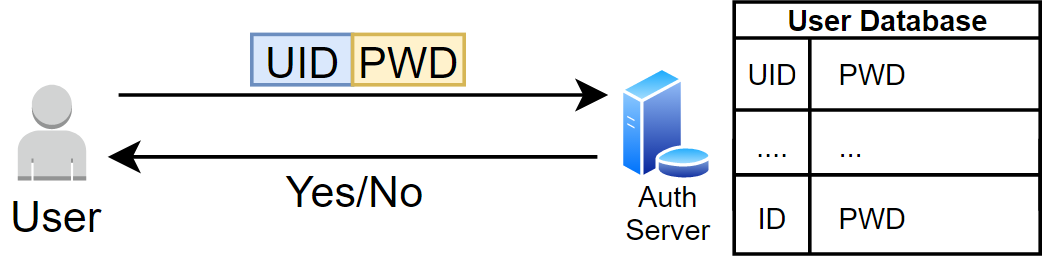
\includegraphics{image/pap.png}
    \caption{PAP scheme}
    \label{fig:pap}
\end{figure}
\begin{note}
\textbf{In PAP le password sono pre-condivise e trasmesse in chiaro ad ogni nuovo tentativo di autenticazione.}
\end{note}\pagebreak
E' facile notare che PAP ha delle limitazioni. In particolare:
\begin{itemize}
    \item  E' soggetto a \textbf{eaves-dropping:}la password e l'ID sono trasmessi in clear, se qualcuno ascolta mette a repentaglio la sicurezza. 
    \item Non c'è protezione da Replay Attack (ad un eventuale attacker basta ascoltare il messaggio che viene inviato all'authenticator per acquisire credenziali valide per entrare). 
    \item Il protocollo non specifica nulla sul numero dei tentativi per entrare (più tentativi a disposizione di un attacker gli garantiscono più possibilità di indovinare).
\end{itemize}
\subsection{Challenge Handshake Authentication Protocol (CHAP)}
Consiste in un approccio più conservativo dal punto di vista della sicurezza, in quanto la password non viene condivisa in chiaro come in PAP (\cref{prop:pap}) ma nascosta tramite una funzione hash.
\begin{remark}
E' necessario porre delle premesse sulla funzione hash usata da CHAP:
\end{remark}
\begin{itemize}
    \item Deve soddisfare le proprietà dei \cref{thm:preimageres,thm:weakcollres,thm:strongcollres}, in particolare la non invertibilità, altrimenti intercettando un messaggio basterebbe applicare la funzione inversa e decifrare la password.
    \item Seguendo le regole degli stream-ciphers, $H(\cdot)$ \textbf{NON} deve essere funzione della sola password $P$. Deve \textbf{SEMPRE} includere qualcosa di \textit{"fresco"}\footnotemark
\end{itemize}
\footnotetext{In genere una \textit{nonce}, ovvero qualcosa di unico, che può essere usato solo una volta.}
\begin{proposition}[CHAP - Challenge Handshake Authentication Protocol]\label{prop:chap}
\begin{enumerate}
    \item L'authenticator invia una \textbf{Challenge} (una \textbf{\textcolor{green}{nonce}}) all'utente, con il compito di \textbf{NON RIPETERE MAI} la challenge inviata.
    \item L'utente risponde con un messaggio contenente lo User ID e una \textbf{Response}:
    \[[UID,H(Challenge, Password, \text{altri oggetti utili}\footnotemark)]\]
    \item L'authenticator cerca nel database l'entry relativa all'UID. Poiché conosce la challenge, è in grado di calcolare l'hash della password e può controllare il valore della response rispetto a quello da lui calcolato. In caso affermativo garantirà l’accesso.
    \footnotetext{\textsuperscript{\thefootnote}Spesso vengono aggiunti altri oggetti utili all'autenticazione, poiché non danneggiano la robustezza della funzione Hash.}
\end{enumerate}
\end{proposition}
\begin{figure}[ht]
    \centering
    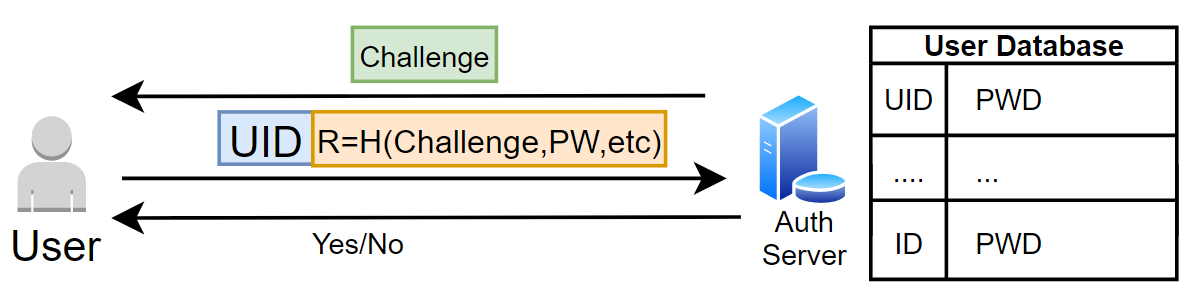
\includegraphics{image/chap.png}
    \caption{CHAP Scheme}
    \label{fig:chap}
\end{figure}
\begin{note}
Poiché abbiamo richiesto che $H(\cdot)$ non sia invertibile, CHAP sfrutta la conoscenza della challenge per consentire l'accesso. Se nella specifica applicazione vengono inviati ulteriori oggetti, l'authenticator dovrà usare anche quelli per calcolare l'hash.
\end{note}
Questo protocollo presenta diversi pro, ma anche un'importante controindicazione:
\begin{itemize}
    \item [\textcolor{green}{\checkmark}]CHAP protegge dai \textbf{replay attacks}, a patto che la challenge non si ripeta mai.
    \item [\textcolor{green}{\checkmark}]Poiché la challenge è decisa dall'ente preposto alla verifica, questo può:
    \begin{itemize}
        \item Controllare la frequenza e la tempistica con cui avvengono le richieste di autenticazione (utile per servizi di banca, ad esempio).
        \item Limitare il tempo di esposizione del sistema ad ogni singolo attacco, ad esempio imponendo un timer tra una richiesta di autenticazione e l'altra.
    \end{itemize}
    \item [\textcolor{red}{\ding{55}}]Il segreto deve essere disponibile nel database in formato plaintext, rendendo \textbf{impossibile} per un sistema che implementa CHAP salvare in DB delle password crittografate in quanto l'hash deve essere irreversibile e soprattutto la nonce deve essere sempre diversa.
\end{itemize}
\subsection{PAP vs CHAP - chi scegliere?}
Nonostante le applicazioni moderne usino PAP, per rispondere correttamente alla domanda su quale sia il miglior protocollo di autenticazione è importante considerare bene i modelli di attacco a cui possono essere sottoposti. 
\begin{theorem}[PAP vs CHAP]
Non esiste un'unica soluzione, \textbf{dipende da quale attacco ci si vuole difendere}.
\end{theorem}
Gli scenari principali sono due:
\begin{enumerate}
    \item \textbf{Attacco al Canale di Comunicazione} (eaves-dropping): Con PAP, è necessaria proteggere il canale di comunicazione\footnotemark \,perché chiunque in ascolto sul canale o chiunque in grado di catturare i pacchetti può conoscere \textit{ID} e \textit{PWD}. \footnotetext{HTTPS, EAP-TTLS, etc} 
    \item \textbf{Attacco al Database Back-End} (Dictionary-Attack to DB): Tipicamente il bersaglio di un sistema di auth sono i sistemi di back-end delle applicazioni, come i database. Se un hacker è in grado di penetrare all'interno del sistema e rubare il DB di password, queste sono esposte nel poiché in chiaro. La soluzione è proteggere le password con un hash, rendendo PAP l'unica soluzione possibile.
\end{enumerate}
Riassumendo: 
\begin{proposition}
CHAP, usando una \textit{nonce} può fare trasmissione in chiaro poiché la password è cifrata.
\end{proposition}
\begin{proposition}
PAP risulta la scelta migliore per difendere i database, perché è possibile nascondere le password con una funzione hash forte e salvare direttamente $H(P)$ piuttosto che la password stessa. Se il DB viene rubato, l'unico modo per bucarlo è facendo brute-force.
\end{proposition}
\begin{note}
Usando password hashate la sicurezza dipende dalla scelta della password, che deve essere forte. 
\end{note}
C'è comunque un modo per proteggere CHAP da attacchi back-end:
\begin{proposition}[CHAP with Explicit Salt]
Supponiamo che il database abbia a disposizione una sorta di chiave numerica, detta \textit{\textbf{Salt}}. Nel suo DB, è salvato l'hash del salto con la password precedentemente scambiata: $H(Salt, Password)$.
\begin{enumerate}
    \item L'authenticator invia una \textbf{Challenge} (\textbf{\textcolor{green}{nonce}}) e il \textbf{Salt} in chiaro all'utente. 
    \item L'utente risponde con un messaggio contenente lo User ID e una \textbf{Response}:
    \[[UID,H(H(Salt, Password),Challenge)]\]
    \item L'authenticator cerca nel database l'entry relativa all'UID. Calcolando l'hash di password e salt insieme alla challenge corrente viene verificato il risultato. In caso affermativo garantirà l’accesso.
\end{enumerate}
Periodicamente e/o se dovesse esserci una falla nella sicurezza, si rigenera il DB con un nuovo Salt. 
\end{proposition}
\begin{remark}
Se un hacker ruba un DB, non può utilizzare la password in quanto è nascosta, ma i dictionary-attack restano comunque validi. 
\end{remark}
\begin{note}Se volessimo usare un database hashato, quale sarebbe la funzione hash da utilizzare? Sappiamo che SHA256 è la migliore al momento, ma presenta 2 problemi dal punto di vista di nascondere delle password:
\begin{enumerate}
    \item E' estremamente veloce: posso crackare l'intero DB più velocemente.
    \item Esiste hardware molto dedicato e specializzato: al 2021 abbiamo 67 TeraHash/s.
\end{enumerate}
Poiché gli attacchi ai DB sono i più comuni, è importante far fronte agli eventuali e successivi brute-force su di essi.
\end{note}\pagebreak
\section{One Time Password (OTP)}
Abbiamo visto che PAP è, generalmente, la scelta più inflazionata per autenticare un utente. OTP si basa sull'idea di migliorare PAP per avere una password diversa ad ogni corretto tentativo di autenticazione. 
\begin{note}
Per prevenire replay attacks, per ogni utente viene memorizzata una password che corrisponde ad un anello di una catena di hash di password. In questo modo viene usata una password sempre diversa ma il database non viene riempito di password per uno stesso utente.
\end{note}
\begin{definition}[Hash Chains Password]
Le password vengono generate applicando più volte una funzione hash a partire dalla password di partenza, garantendo che la password sarà sempre diversa da quella usata in un precedente tentativo di autenticazione terminato con successo.
\end{definition}
\begin{remark}
Non stiamo risolvendo il problema dell'eavesdropping, in quanto una volta intercettata una delle password, un attaccante sarà in grado di generare anche tutte le successive. Inoltre, bisogna gestire dei meccanismi di perdita di pacchetti, inserendo delle finestre di tolleranza nei protocolli, ma come scegliamo la dimensione della finestra?
\end{remark}
\begin{proposition}[OTP - One Time Password]\label{prop:otp}
\begin{enumerate}
    \item L'authenticator scambia $P[0]$ con il client e genera $N+1$ password a partire da $P[0]$ calcolando:
    \begin{equation*}
        P[i]=H(P[i-1])
    \end{equation*}
    Nel database salverà soltanto la password $P[N+1]$
    \item L'utente genera $N$ password a partire da $P[0]$, seguendo la stessa logica.
    \item L'utente procede all'autenticazione secondo PAP (\cref{prop:pap}), inviando le password a partire dall'ultima generata: \textit{(UID,P[N])}
    \item L'authenticator controlla se $H(P[N])==P[N+1]$. Se vero, sovrascrive nel DB la password con $P[N]$ e invia un messaggio di avvenuta autenticazione. Altrimenti invia un messaggio di rifiuto.
\end{enumerate}
\end{proposition}
  \begin{note}
    Durante l'autenticazione i-esima, la password salvata nel DB è $P[i]$, pertanto il controllo sarà: $H(P[i])==P[i-1]$
    \end{note}
\begin{remark}
Capiamo che in OTP, se un tentativo di autenticazione va a buon fine, viene salvata sempre la password \textbf{PRECEDENTE} a quella attualmente presente nel database.
\end{remark}
Riassumendo, vantaggi e svantaggi sono: 
\begin{itemize}
    \item [\textcolor{green}{\checkmark}]Ad ogni autenticazione viene eseguita una sola hash.
    \item [\textcolor{green}{\checkmark}]Il DB memorizza un solo valore per utente.
    \item [\textcolor{green}{\checkmark}]Robustezza contro attacchi server-side (è impossibile prevedere pwd precedenti).
    \item [\textcolor{green}{\checkmark}]Le password possono essere trasmesse in chiaro sul canale.
    \item [\textcolor{red}{\ding{55}}]Serve un grande valore di n per evitare di finire le password a disposizione (servirà una nuova registrazione dopo).
    \item [\textcolor{red}{\ding{55}}]Vulnerabilità lato client (tiene memorizzato il seed della password).
    \item [\textcolor{red}{\ding{55}}]Possibilità di desincronizzazione (se per qualche motivo fallisce un accesso, si perde la catena, in quanto l'utente la volta dopo proverà ad entrare con p[n-1] in giù, mentre l'authenticator si aspetta ancora p[n]).
\end{itemize}
\section{Two-Factor Authentication}
Assumiamo che sia client che server siano entità sicure e non penetrabili e che l'autenticazione avvenga attraverso l'ausilio di una password e di un oggetto aggiuntivo come un \textit{One Time Authorization Token} (generato su un device differente o ricevuto su un canale differente, come e-mail, SMS etc), di lunghezza pari a 6/8 cifre (quindi serve una hash in grado di troncare la lunghezza).\\
Ci sono due protocolli per un sistema 2FA:
\begin{proposition}[HOTP - Hash based OTP]\label{prop:hotp}
\begin{itemize}
    \item [\textbf{idea:}]Basato sull'utilizzo di un contatore $N$.
\end{itemize}
Sul server e sul client è memorizzata una secret-key, la password è calcolata come: 
\begin{equation*}
    P[N]=H[K,N]
\end{equation*}
La password generata non è più una catena in quanto ogni volta il contatore cambia e il bitstream da hashare è sempre diverso.
\end{proposition}
\begin{note}
Anche se un attaccante dovesse conoscere $P[N]$, non potrebbe calcolare $P[K,N+1]$.
\end{note}
\begin{note}
La password n-esima può essere calcolata in modo asincrono, purché sia nota la chiave di partenza.
\end{note}
\begin{note}
La differenza con il OTP (\cref{prop:otp}) è che la password non è più pre-calcolata in ordine inverso. 
\end{note}
\begin{proposition}[TOTP - Time based OTP]\label{ prop:totp}
Simile a HOTP (\cref{prop:hotp}) ma il contatore è il tempo.
\end{proposition}
\begin{note}
Un possibile attacco potrebbe essere effettuato, sfruttando la possibilità che un attaccante possa manipolare il tempo registrato nella macchina, controllando di fatto il token.
\end{note}
\begin{corollary}
Come "esperti di sicurezza" vorremmo che un sistema 2FA sia sempre implementato e sempre utilizzato, in quanto rappresenta una protezione aggiuntiva difficilmente aggirabile dato che sfrutta un canale di comunicazione diverso.
\end{corollary}
\section{Mutual Authentication}\label{chap:mutualauth}
Nei protocolli descritti sopra abbiamo trattato come "entità poco sicura" esclusivamente l'utente. Tuttavia, in un contesto reale è molto utile \textbf{verificare la legittimità dell'entità a cui ci connettiamo}.\\
Un possibile modo di fare mutua autenticazione è quello di usare CHAP (\cref{prop:chap}). L'idea consiste in:
\begin{enumerate}
    \item Il server invia la challenge e l'utente risponde con \textit{(ID, H(shared-key, challenge))}. Dopo i controlli, il server invia un \textit{ACK} per indicare il successo dell'auth.
    \item L'utente invia una nuova challenge e il server risponde con \textit{(ServerName, H(shared-key, new-challenge))}. Dopo i controlli, l'utente invia un \textit{ACK} al server per indicare il successo dell'auth.
\end{enumerate}
\begin{figure}[h]
    \centering
    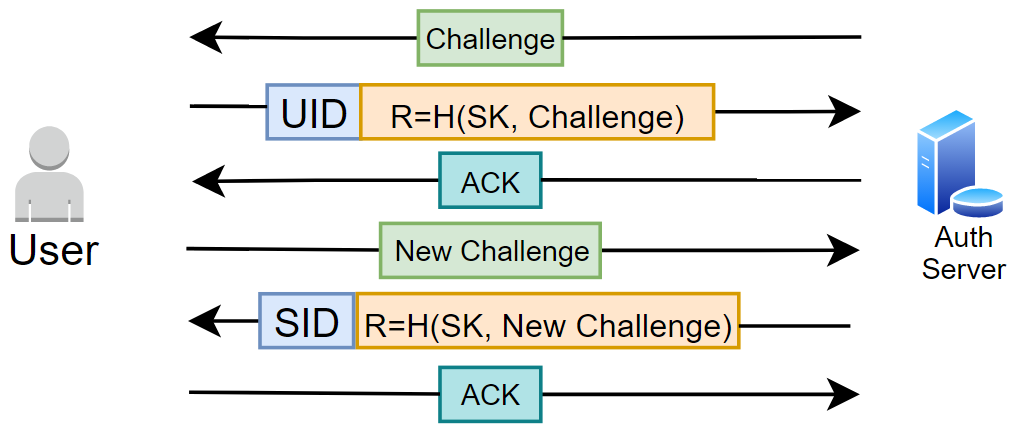
\includegraphics[width=0.9\textwidth]{image/chapmutual.png}
    \caption{Mutual Auth with Chap}
    \label{fig:chapmutual}
\end{figure}
\begin{remark}
L'idea di base non pone restrizioni sull'effettiva sequenza di messaggi che devono essere scambiati, questo pone un attaccante in posizione di vantaggio (\cref{fig:chapmutualatk}). Difatti, l'hacker potrebbe inoltrare al server la stessa challenge e lui dovrebbe rispondere con il suo nome e l'hash della challenge. A questo punto l'hacker si è mostrato legittimo per il server e può autenticare la sua identità digitale inoltrando la response precedente. 
\end{remark}
\begin{figure}[h]
    \centering
    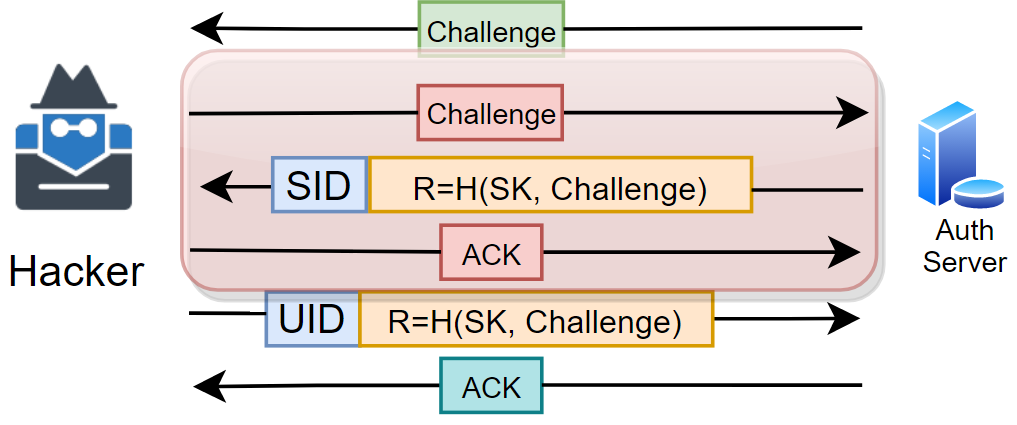
\includegraphics[width=0.9\textwidth]{image/chapmutualatk.png}
    \caption{Mutual Auth attack scheme}
    \label{fig:chapmutualatk}
\end{figure}
Lo schema precedente non è il solo attacco che diventa disponibile adesso, perché ora il sistema è soggetto al \textit{reflection attack}
\begin{definition}
[Reflection Attack]\label{def:reflectionatk}
L'attaccante è in grado di fingersi come access point. A questo punto può farsi inviare da un utente un messaggio con il quale può verificare la sua identità digitale. Lo schema è il seguente (\cref{fig:reflectionatk}): 
\begin{enumerate}
    \item A si finge access point ed invia una challenge $C_1$ ad U. 
    \item U invia la sua challenge $C_2$ (per autenticare l'altro end-point) e la sua response.\label{resp}
    \[(\text{UID}, H(K,C_1))\]
    \item A \textbf{ignora la response} e inoltre ad U la sua stessa challenge: (AID, $C_2$).
    \item U risponde di nuovo come al punto \ref{resp} con $C_2$ al posto di $C_1$
    \item A può autenticarsi, rispondendo con (AID, H(K,$C_2$))
\end{enumerate}
\end{definition}
\begin{figure}[h]
    \centering
    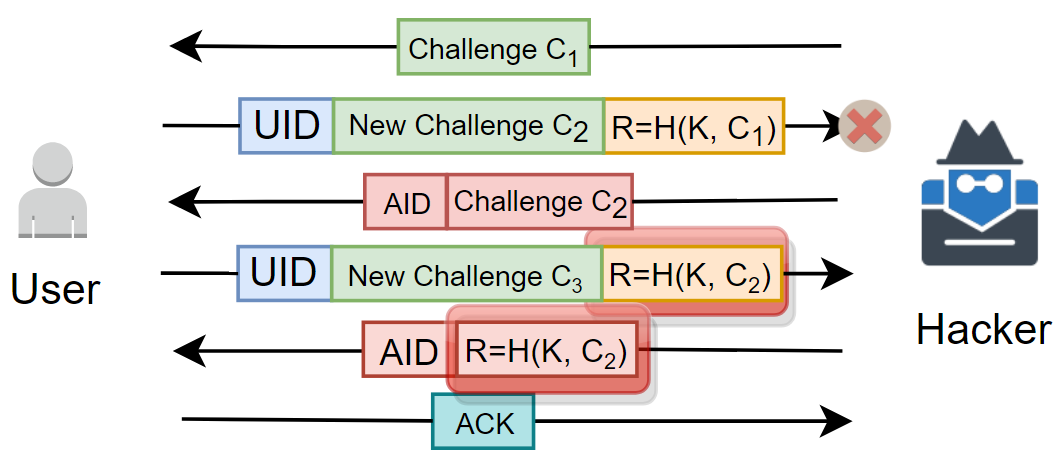
\includegraphics[width=0.9\textwidth]{image/reflectionatk.png}
    \caption{Reflection Attack in Mutual Auth}
    \label{fig:reflectionatk}
    \vspace{5pt}
\end{figure}
\subsection{Come prevenire Reflection Attacks?}
Un modo per impedire che le challenge siano riflesse, è tenere traccia della precedente challenge e dell'ordine con cui vengono inviate e calcolare l'hash di quella coppia come response. In questo modo anche osservando le challenge, un attaccante non potrà autenticarsi in quanto senza shared secret non potrà calcolare delle response valide. Lo schema, riportato in \cref{fig:reflectionavoid}, è:
\begin{enumerate}
    \item L'authenticator invia (SID, $C_1$).
    \item U genera $C_2$ ed invia (UID, $C_2$, H(K, $C_1$)). L'authenticator conosce l'ordine e può autenticare U.
    \item L'authenticator risponde con (SID, H(K, $C_1$, $C_2$)). U conosce l'ordine e può autenticare il server.
\end{enumerate}
\begin{figure}[ht]
    \centering
    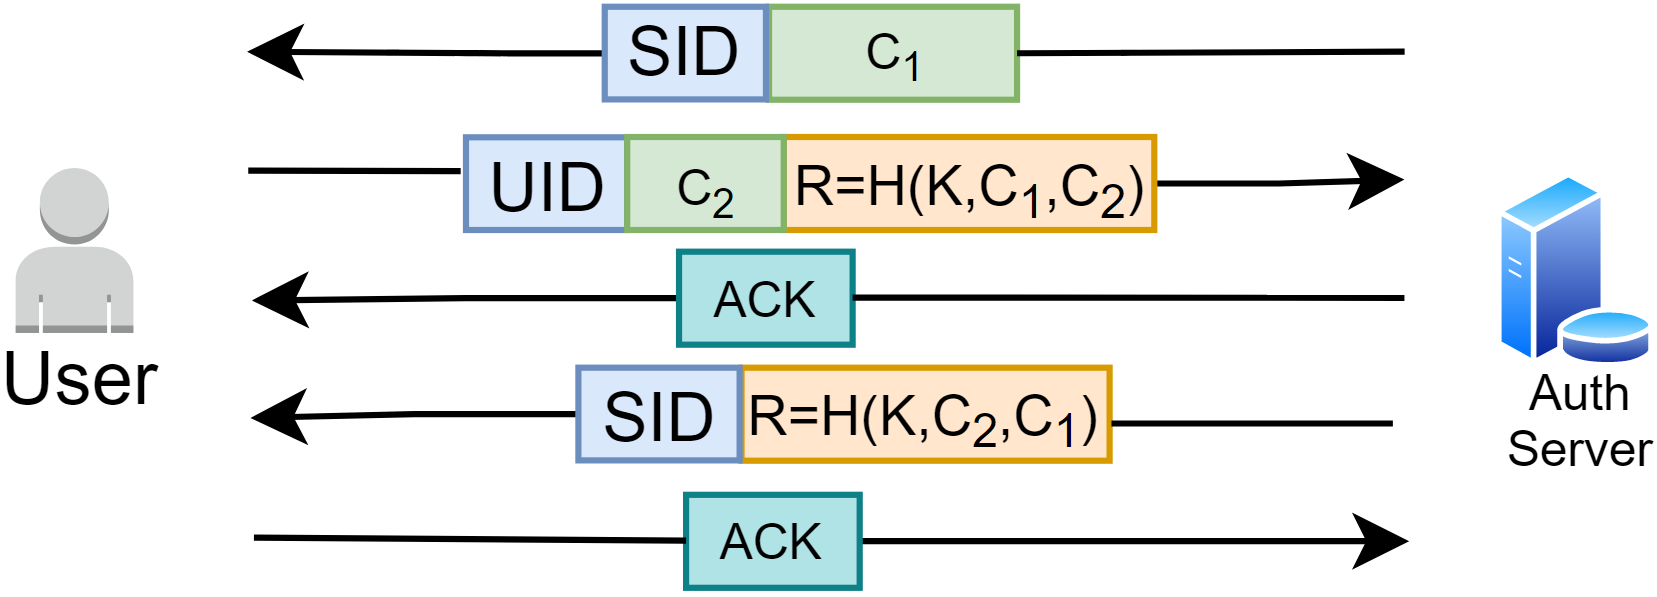
\includegraphics[width=0.8\textwidth]{image/reflectionavoid.png}
    \caption{Avoid Reflection Attack Scheme}
    \label{fig:reflectionavoid}
\end{figure}
\begin{corollary}[Lo scopo di un protocollo]
Mai usare un algoritmo per un obiettivo che non è quello per cui è stato pensato
\end{corollary}
La mutua autenticazione con CHAP è sbagliata di fondo, in quanto è un algoritmo pensato per essere \textit{"Single-Side authentication"}, mentre noi lo stiamo forzando a lavorare in un contesto \textit{"Dual-Side"}. Infatti, i reflection attacks ci sono ogni qualvolta usiamo uno stesso protocollo per autenticare due end-point. 
\begin{note}
Un protocollo di mutua autenticazione non può autenticare indipendentemente le due parti, in quanto espone vulnerabilità per il sistema. L'unico modo per eseguire il processo correttamente è quello di \textbf{legare insieme} le due challenge crittografandole in una unica response.
\end{note}
